% *******************************************************************************
% * Copyright (c) 2007 by Elexis
% * All rights reserved. This document and the accompanying materials
% * are made available under the terms of the Eclipse Public License v1.0
% * which accompanies this distribution, and is available at
% * http://www.eclipse.org/legal/epl-v10.html
% *
% * Contributors:
% *    G. Weirich - initial implementation
% *
% *  $Id: stammdaten.tex 3569 2008-01-21 17:55:22Z rgw_ch $
% *******************************************************************************
% !Mode:: "TeX:UTF-8" (encoding info for WinEdt)

\section{Stammdaten-Views}

\subsection{Patienten}
\index{Patientenliste}
Die Patientenliste dient sowohl der Anzeige existierender Patienteneinträge, als
auch dem Erfassen neuer Einträge. Die Liste zeigt all diejenigen Kontakte an,
die als Patient markiert sind.
\begin{figure}[ht]
	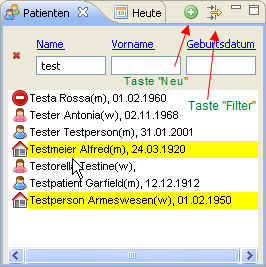
\includegraphics{images/patlistview}
	\caption{Patientenliste}
	\label{fig:patlist}
\end{figure}
Die Eingabefelder oben (Name, Vorname, Geburtsdatum) dienen dem Filtern der
Liste gemäss den gewünschten Parametern.
\begin{itemize}
  \item Bei Name und Vorname gilt:
	\begin{itemize}
      \item Wenn Sie mindestens zwei Buchstaben eingeben, erscheinen in der
      Liste nur noch diejenigen Einträge, die mit diesen Buchstaben \textit{beginnen}.
      \item Wenn Sie das Zeichen \% und mindestens zwei weitere Buchstaben
      eingeben, dann erscheinen in der Liste diejenigen Einträge, die diese
      Zeichenfolge \textit{enthalten}.
    \end{itemize}
  \item Beim Geburtsdatum gilt:
	\begin{itemize}
      \item Wenn Sie mindestens 3 aufeinanderfolgende Ziffern eingeben, dann wird
      die Zahl als Jahreszahl interpretiert und es werden diejenigen Patienten
      ausgewählt, die das entsprechende \textit{Geburtsjahr} haben.
      \item Wenn Sie zwei Ziffern, gefolgt von einem Punkt und ggf. weitere 2
      Ziffern eingeben, dann werden diejenigen Patienten angezeigt, die den
      entsprechenden \textit{Geburtstag} und ggf. \textit{Geburtsmonat} haben.
      Beachten Sie bitte, dass Sie Tag und Monat zweistellig eingeben müssen,
      also z.B. 04.05. und nicht etwa 4.5.
     \end{itemize}
\end{itemize}
Wenn keine Einträge existieren, die den eingegebenen Filterbedingungen
entsprechen, dann wird in der Liste angezeigt: \glqq keine Daten\grqq.
\subsubsection{Toolbar}
\begin{itemize}
  \item Mit der Taste \glqq Neu\grqq{} (s. Abb. \ref{fig:patlist}) können Sie
  einen neuen Patienten erfassen. Klick
  auf diesen Knopf öffnet die Patienteneingabe-Dialogbox. Diejenigen Felder, die
  Sie bereits eingegeben haben, sind vorgegeben, die anderen können Sie soweit
  eingeben, wie sie im Moment bekannt sind. Mit Klick auf \glqq OK\grqq{}wird
  der neue Patienteneintrag angelegt. Bei Klick auf \glqq Abbrechen\grqq{}werden
  die eingegebenen Daten verworfen und es wird kein neuer Eintrag erstellt.
  Falls ein neuer Eintrag erstellt werden soll, und bereits ein Eintrag mit
  gleichen Daten existiert, dann erfolgt eine Rückfrage.

  \item Mit der Taste \glqq Filter\grqq{} (s. Abb. \ref{fig:patlist}) können Sie
  die Liste nach
  verschiedenen Kriterien filtern (s. Abb. \ref{fig:patlistfilter}).
	\begin{figure}[ht]
    	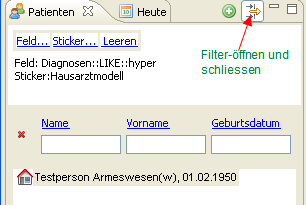
\includegraphics{images/patlistfilter}
    	\caption{Filterbedingungen eingeben}
    	\label{fig:patlistfilter}
    \end{figure}
	\textbf{Achtung}: Der Filter rastet ein und wird erst wieder aufgehoben, wenn
	Sie erneut auf den Filter-Knopf klicken. Solange er eingerastet ist, wirken
	alle anderen Eingaben nur auf die bereits gefilterte Auswahl.
\end{itemize}
\subsubsection{View-Menü}
Das lokale Menü (s. Abb. \ref{fig:patlist}) enthält folgende Einträge:
\begin{itemize}
  \item Patient löschen (sofern der angemeldete Anwender die hierfür notwendigen
  Rechte hat): Damit kann ein Patienteneintrag definitiv und unwiderruflich aus
  der Datenbank gelöscht werden. Dies ist nur dann möglich, wenn zu diesem
  Patienten keine Fälle (mehr) existieren.
  \item Liste filtern: Dies öffnet ebenfalls die Filter-Dialogbox (s.o.)
\end{itemize}

\subsubsection{Kontextmenü}
Das Kontextmenü erscheint, wenn Sie auf einem Pa\-tien\-ten\-eintrag mit der rech\-ten
Maus\-taste klicken. Es enthält fol\-gende Ein\-träge:
\begin{itemize}
  \item Patient löschen (s. oben)\footnote{Sie benötigen dazu das Recht \textsc{Löschen/Kontakt} (Vgl. \ref{sec:gruppen})}
  \item KG exportieren. Falls ein Export-Plugin installiert ist, wird die KG des
  aktuell markierten Patienten über dieses Plugin exportiert. Falls mehrere
  Export-Plugins definiert sind, erscheint zunächst eine Dialogbox, mit der sie
  das ge\-wünschte Ziel bzw. Format auswählen können.\footnote{Sie benötigen dazu das Recht \textsc{Daten/Kontakt/exportieren}}
\end{itemize}


\subsection{Patient-Detail}
\index{Patient!Detailangaben}
Diese View (Abb. \ref{fig:patdetail} zeigt Details des momentan ausgewählten
Patienten resp. der momentan ausgewählten Patientin an
 %\usepackage{graphics} is needed for \includegraphics
\begin{figure}[htp]
\begin{center}
  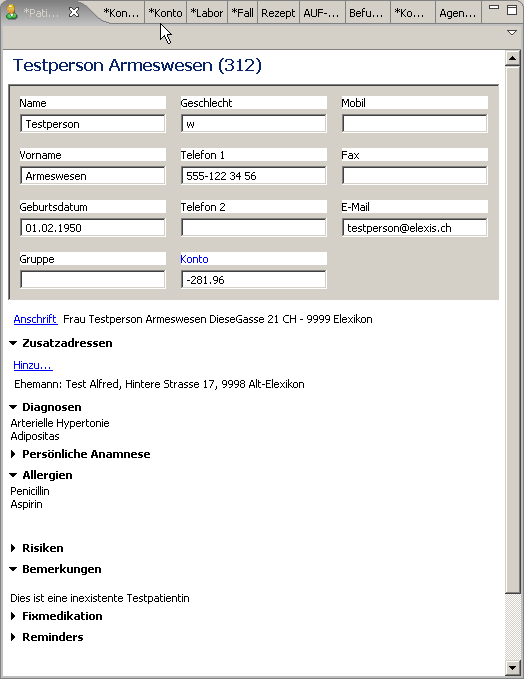
\includegraphics[width=0.9\textwidth]{images/patdetail}
  \caption{Patient Detailansicht}
  \label{fig:patdetail}
\end{center}
\end{figure}
Alle Felder können durch einfaches Überschreiben geändert werden, sofern der
aktuell eingeloggte Anwender die dazu erforderlichen Rechte besitzt. Eine
Änderung wird in dem Moment gespeichert, in dem ein Feld wieder verlassen wird.
(Explizites Speichern ist in Elexis nie notwendig).

Die Felder im oberen Block sind alle einzeilige Textfelder und können direkt geändert
werden, bis auf das Feld \glqq Konto\grqq{}, welches nicht direkt beschreibbar
ist. Dieses Feld stellt den Saldo aller Forderungen an diesen bzw. Zahlungen von
diesem Patienten dar. Wenn der aktuell eingeloggte Anwender Verrechnungs-Rechte
besitzt, kann er den blauen Text \glqq Konto\grqq{} anklicken, dann öffnet sich
ein Dialog, in dem einzelne Buchungen eingegeben werden können.

\textbf{Achtung}: Normalerweise erfolgen Buchungen automatisch durch Erstellen
von Rechnungen und Einlesen von ESR-Files. Manuelle Buchungen können zu
Inkonsistenzen in der Buchhaltung führen. Führen Sie also nur dann manuelle
Buchungen durch, wenn Sie sich über die Konsequenzen exakt bewusst sind.

Das Feld \glqq Anschrift\grqq{} zeigt die Postanschrift des Patienten an. Diese
kann durch Klick auf den blauen Text \glqq Anschrift \grqq{}geändert werden.

Die darunterstehenden Felder sind alle aufklappbar: Standardmässig ist nur der
Titel sichtbar, durch Klick darauf öffnet sich das Feld.
\begin{itemize}
  \item Das Feld \glqq Zusatzadressen\grqq{}dient dazu, Kontakte, die in
  irgendeiner Beziehung zum Patienten stehen, zu erfassen. Beispielsweise
  Angehörige, Ämter, weitere Ärzte etc. Klick auf \glqq Hinzu\grqq{} öffnet eine
  Kontaktauswahl-Box, aus der die gewünschte Person oder Organisation ausgewählt
  werden kann. Danach erscheint eine Eingabebox, in der die Beziehung des eben
  ausgewählten Kontakts zum Patienten beschrieben werden kann. \\
  Mit Rechtsklick auf einen Eintrag in diesem Feld öffnet sich ein Kontextmenü,
  mit dem man den vollständigen Eintrag anzeigen, oder den Eintrag entfernen kann.
  \item Die Felder \glqq Diagnose\grqq, \glqq Persönliche Anamnese\grqq{},
  \glqq Allergien\grqq{}, \glqq Risiken\grqq{} und \glqq Bemerkungen \footnote{Falls in \textit{Bemerkungen} irgendwo :VIP: (mit den Doppelpunkten) steht, so wird der betreffende Pat. in roter Schrift angezeigt.}\grqq{}
  können direkt beschrieben werden und werden wie gewohnt sofort beim Verlassen
  gespeichert.
  \item Das Feld \glqq Fixmedikation\grqq{}entspricht der View Fixmedikation.
  \item Das Feld \glqq Reminders\grqq{} zeigt die Reminders zum aktuellen Patienten.
\end{itemize}
\subsection{Kontakte}
Diese View (Abb. \ref{fig:kontaktlist}) zeigt eine Liste aller in Elexis
vorhandenen Kontakte an. Ein Kontakt
ist jede Person oder jede Organisation, welche in irgendeiner Beziehung zu
unserer Praxis steht. Das sind beispielsweise Patienten, Kollegen, Spitäler,
Versicherungen, Labors, Lieferanten usw.
%\usepackage{graphics} is needed for \includegraphics
\begin{figure}[htp]
\begin{center}
  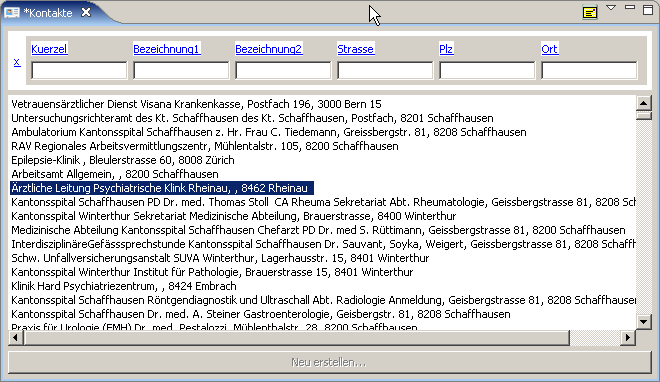
\includegraphics[width=0.9\textwidth]{images/kontaktlistview}
  \caption{Kontaktliste-View}
  \label{fig:kontaktlist}
\end{center}
\end{figure}
Mit Klick auf das Briefumschlag-Symbol rechts oben können Sie eine
Adressetikette für den betreffenden Kontakt ausdrucken.

\subsection{Kontakt-Detail}
Hier werden die Details zum aktuell ausgewählten Kontakt angezeigt und können
geändert werden (Abb. \ref{fig:kontaktdetail}).
%\usepackage{graphics} is needed for \includegraphics
\begin{figure}[htp]
\begin{center}
  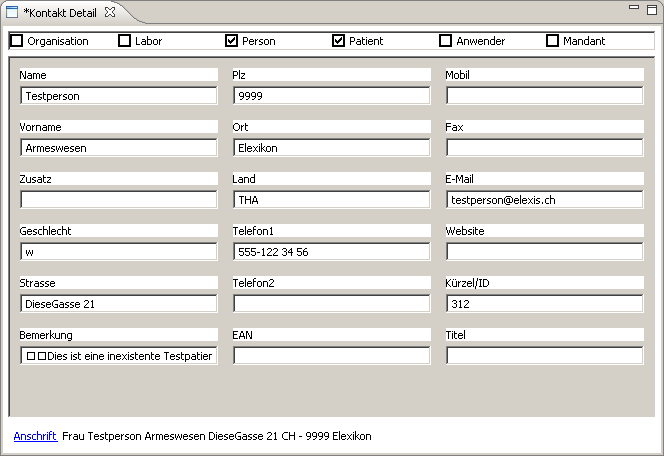
\includegraphics[width=0.9\textwidth]{images/kontaktdetail}
  \caption{Kontakt Detailview}
  \label{fig:kontaktdetail}
\end{center}
\end{figure}
In den Checkboxen der obersten Zeile können Sie den Typ des betreffenden
Kontakts festlegen. Beachten Sie, dass ein Kontakt auch mehrere Typen haben kann
(Beispielsweise kann jemand Anwender und auch Patient sein). Hingegen kann
ein Kontakt natürlich nur entweder eine Organisation oder aber eine Person sein.
Achten Sie darauf, dies und bei Personen auch das Geschlecht (m oder w) korrekt
zu erfassen, da Textformatvorlagen diese Informationen auswerten, um die
korrekten Formulierungen auszuwählen.

In der untersten Zeile steht die Postanschrift des betreffenden Kontakts. Dies
ist die Adresse, wie sie beispielsweise im Adressfeld von Briefen oder
Rechnungen oder auf Adressetiketten erscheinen soll. Mit Klick auf das blaue
Wort \glqq Anschrift\grqq{}öffnet sich die Anschrifteingabe-Dialogbox (Abb.
\ref{fig:anschrift}), wo Sie beliebigen Text eingeben können. (Klick auf den
Button \glqq Postanschrift\grqq{} erstellt eine Standard-Anschrift aus den
vorhandenen Adressangaben)


\begin{figure}[htp]
\begin{center}
  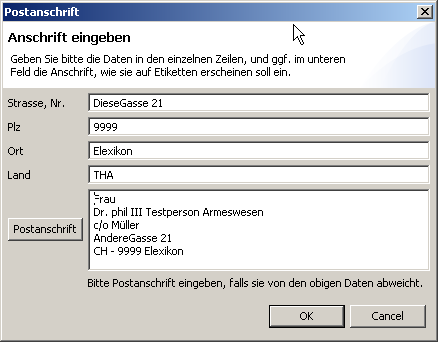
\includegraphics{images/anschrifteingabe}
  \caption{Anschrift-Eingabe}
  \label{fig:anschrift}
\end{center}
\end{figure}
\bigskip
\pagebreak[3]
\subsection{Artikel}
\label{view:artikel}
\index{Artikel}
Ein \glqq Artikel\grqq{}ist jedes Objekt, das auf Lager genommen und/oder
abgegeben werden kann. Es gibt einerseits vordefinierte Artikel (z.B. die Liste
aller zugelassenen Medikamente), andererseits auch Eigenartikel. Elexis kann den
Lagerbestand von Lagerartikeln verwalten und halbautomatisch Bestellungen zur Neige
gehender Artikel vornehmen.


\subsection{Artikelliste}
In Abb. \ref{fig:artikel} ist eine Artikelauswahl-Liste und die
Artikeldetaildarstellung nebeneinander zu sehen.

 %\usepackage{graphics} is needed for \includegraphics
\begin{figure}[htp]
\begin{center}
  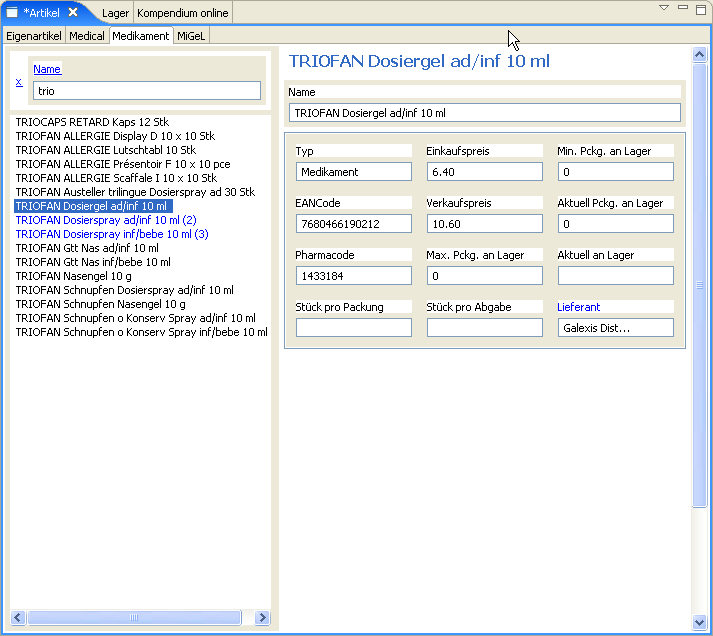
\includegraphics[width=0.9\textwidth]{images/artikelview}
  \caption{Artikel-View}
  \label{fig:artikel}
\end{center}
\end{figure}
Die Liste links können Sie in gewohnter Weise filtern, indem Sie einige
Buchstaben des gewünschten Artikelnamens eingeben.
In der Detailansicht sehen Sie Einzelheiten zum gerade ausgewählten Artikel. (In
Perspektiven, wo die Liste allein dargestellt ist, können Sie mit der rechten
Maustaste und \glqq Bearbeiten\grqq{} zur Detailansicht gelangen.)

\index{Lager}
Ein Artikel wird dadurch zum Lagerartikel, dass Sie ihm einen Mindestbestand
grösser als Null zuweisen. Geben Sie ausserdem einen Höchstbestand höher als der
Mindestbestand ein und weisen Sie dem Feld \glqq Istbestand\grqq{} den korrekten
Wert zu. Elexis wird bei einer halbautomatischen Bestellung von jedem Artikel,
dessen Istbestand unter dem Mindestbestand ist, soviele Exemplare bestellen, um
auf den Höchstbestand zu kommen.

Bei manchen Artikeltypen wird üblicherweise nicht eine ganze Verpackungseinheit
auf einmal abgegeben, beispielsweise Ampullen. Hierfür sind die Felder \glqq
Stück pro Packung\grqq{}und \glqq Stück pro Abgabe\grqq{}vorgesehen. Angenommen
ein Artikel wird in Packungen zu 10 Stück eingekauft, aber einzeln abgegeben.
In diesem Fall können Sie bei Stück pro Abgabe eine 1 setzen, bei Stück pro
Packung eine 10. Wenn dieser Artikel dann einem Patienten verrechnet wird, dann
wird automatisch 1/10 des Verpackungs-Verkaufspreises berechnet und auch nur
1/10 einer Packung aus dem Lager ausgebucht.

Die Angabe \glqq Aktuell an Lager\grqq{} meint dann die Zahl der einzelnen
Artikel, während \glqq Aktuell Pck. an Lager\grqq{} für die Zahl der
unangebrochenen Packungen steht.


\subsection{Lager und Bestellung}
\index{Artikel!bestellen}
Wie oben beschrieben, kann Elexis Ihr Warenlager halbautomatisch bewirtschaften.
Wann immer Sie einem Patienten einen Artikel verrechnen, wird dieser Artikel
automatisch aus dem Lagerbestand ausgebucht. Sobald der Bestand eines
Lagerartikels unter den von Ihnen definierten Mindestbestand fällt, \glqq
weiss\grqq{} Elexis, dass dieser Artikel nachbestellt werden muss. Nebst dieser
automatischen Erkennung können Sie selbstverständlich Bestellungen auch manuell
erstellen und/oder ändern.

Diese Funktionen sind in der View \glqq Bestellung\grqq{} erreichbar (s. fig.
\ref{fig:bestellungen}).
 %\usepackage{graphics} is needed for \includegraphics
\begin{figure}[htp]
\begin{center}
  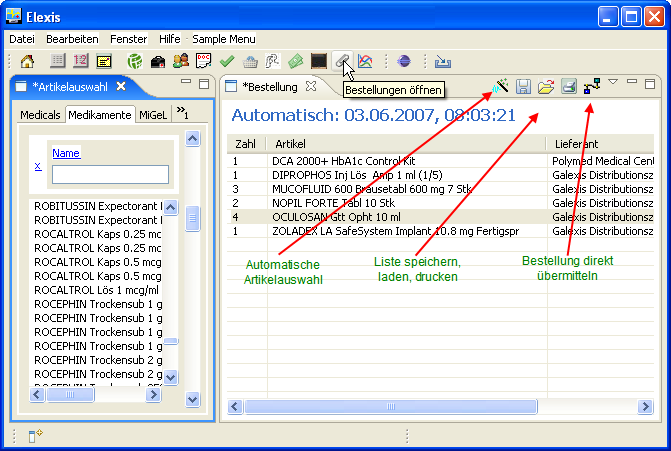
\includegraphics[width=0.9\textwidth]{images/bestell1}
  \caption{Bestellungen - View}
  \label{fig:bestellungen}
\end{center}
\end{figure}


Links finden Sie die schon bekannten Artikelauswahlfenster für alle
Artikelkategorien, für die Sie Plugins haben (Normalerweise Medikamente,
Medicals, MiGeL und Eigenartikel). Rechts ist das Feld Bestellung, welches
anfangs leer ist. Sie haben nun folgende Möglichkeiten:
\begin{itemize}
  \item Mit Klick auf das Zauberstab-Symbol werden automatisch diejenigen
  Artikel der Bestellung zugefügt, von welchen weniger als der Mindestbestand an
  Lager ist. Es werden jeweils soviele bestellt, dass der für diesen Artikel
  definierte Höchstbestand erreicht wird.
  \item Sie können aus einem der Fenster links Artikel in die Bestellung
  herüberziehen.
	\item Sie können auf einen der Artikel in der Bestelliste mit der rechten
	Maustase klicken, und den Artikel aus der Liste entfernen oder die Zahl ändern.
	
	\item Sie können die Bestellung erst mal abspeichern und später weiterbearbeiten.
	
	\item Sie können eine früüher gespeicherte Bestellung wieder laden.
	\item Sie können die Bestellung ausdrucken. Dafür ist eine System-Textvorlage (s. S.
	\pageref{textvorlagen}) namens \glqq Bestellung\grqq{} notwendig, welche an
	einer Stelle den Platzhalter [Bestellung] enthält (s. Abb. \ref{fig:bestell2}).
	\item Last but not least können Sie, falls Sie ein entsprechendes Plugin für
	Ihren Lieferanten haben, die Bestellung direkt via Internet oder Modem
	absenden. Ein entsprechendes Plugin für Galexis ist bereits verfügbar, weitere
	werden entwickelt.
\end{itemize}
\begin{figure}[hb]
  % Requires \usepackage{graphicx}
  
\includegraphics{images/bestell2}\\
  \caption{Ausschnitt aus der Vorlage Bestellung}\label{fig:bestell2}
\end{figure}

\subsection{codes}
Codes



